% !TEX root = ../thesis-sample.tex

\chapter{Introduction} \label{chap:intro}

Here's an acronym \ac{CRTBP}
\section{Float environments}
Theere are many possible float enviornments, and this section will serve as an introduction and demonstration of each of them.
In addition, it offers the ability to ensure that this template actually follows the guidelines.

\subsection{Figures}\label{ssec:figures}


Here is a figure as shown in~\cref{fig:plain}.

\begin{figure}
    \centering
    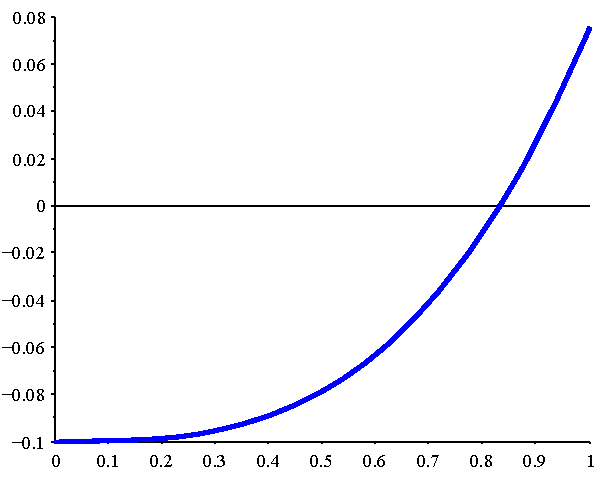
\includegraphics[width=0.5\textwidth]{figures/f1_plain.pdf}
    \caption[Short caption for TOC]{Long caption to appear in text\label{fig:plain}}
\end{figure}

\subsection{Tables}\label{ssec:tables}

here's a table in~\cref{tab:table}

\begin{table}
\begin{center}
    \begin{tabular}{ | l | l | l | p{5cm} |}
    \hline
    Day & Min Temp & Max Temp & Summary \\ \hline
    Monday & 11C & 22C & A clear day with lots of sunshine.  
    However, the strong breeze will bring down the temperatures. \\ \hline
    Tuesday & 9C & 19C & Cloudy with rain, across many northern regions. Clear spells 
    across most of Scotland and Northern Ireland, 
    but rain reaching the far northwest. \\ \hline
    Wednesday & 10C & 21C & Rain will still linger for the morning. 
    Conditions will improve by early afternoon and continue 
    throughout the evening. \\
    \hline
    \end{tabular}
    \caption[Short caption for table]{Long caption for text \label{tab:table}}
    \end{center}
\end{table}

\section{References and Citation}

\subsection{Clever referencing}
\LaTeX offers the powerful ability to automatically handle references using \verb+\label+ and a corresponding \verb+\ref+.
While~\cref{chap:intro} has more detail on some good practices for \LaTeX~that I've picked up.

\subsection{References}

We can cite lots of useful papers~\cite{bhat2000,chaturvedi2011a}.

\section{Math}

Here are some nice equations~\cref{prob_def,prob_def_constrained}

\begin{align}
\label{prob_def}
&\min_{s\subset W}\ J(s) = \sum_{i=1}^{l-1} H(s_j, s_{j+1}) \\
&\max_{s\subset W}\ P_{tr}(s) = \prod_{i=1}^{l-1} P_{tr}(s_j, s_{j+1}) \nonumber
\end{align}

\begin{align}
\label{prob_def_constrained}
&\min_{s\subset W}\ J(s) = \sum_{i=1}^{l-1} H(s_j, s_{j+1}) \\
&\text{subject to} \ P_{tr}(s)>\epsilon_{tr} \nonumber
\end{align}
